% Copyright 2005-2016 Airbus-EDF-IMACS-Phimeca.
% Permission is granted to copy, distribute and/or modify this document
% under the terms of the GNU Free Documentation License, Version 1.2
% or any later version published by the Free Software Foundation;
% with no Invariant Sections, no Front-Cover Texts, and no Back-Cover
% Texts.  A copy of the license is included in the section entitled "GNU
% Free Documentation License".

The \OT\ project is an open source project. It aims at developing a computational platform designed to carry out industrial studies on uncertainty processing and risk analysis.

This platform is intended to be released as an open source contribution to a wide audience whose technical skills are very diverse. Another goal of the project is to make the community of users ultimately responsible for the platform and its evolution by contributing to its maintenance and developing new functions.

This architecture specifications document therefore serves two purposes:
\begin{itemize}
\item to provide the design principles that govern the platform, in order to guide the development teams in their development process;
\item to inform external users about the platform's architecture and its design, in order to facilitate their first steps with the platform.
\end{itemize}

% In the first section of this document, we will introduce the concepts that governed the construction of the platform. These concepts resulted from the requirements analysis carried out with the users and the developers, following the UML approach. The general functions of the platform allowed us to categorize the concepts by giving us a more synthetic and global view of its components.
%
%
% The second section details the technical choices that were retained for the platform's development.

To address these questions, the \OT\ platform needs to be:
\begin{itemize}
\item \emph{portable}: the ability to build, execute and validate the application in different environments (operating system, hardware platform as well as software environment) based on a single set of source code files.
\item \emph{extensible}: the possibility to add new functions to the application with a minimal impact on the existing code.
\item \emph{upgradable}: the ability to control the impact of a replacement or a change on the technical architecture, following an upgrade of the technical infrastructure (such as the replacement of one tool by another or the use of a new storage format).
\item \emph{durable}: the technical choices must have a lifespan comparable to the application's while relying on standard and/or open source solutions.
\end{itemize}


\subsection{Overview}

This chapter will describe the general design of \OT\, and a few design models that are widely used within the platform.

The core of OpenTURNS platform is a C++ library made of about 500 classes of various size.

The main user interface is a python module, automatically generated from the C++ library using the wrapping software SWIG. It allows for a usage of OpenTURNS through python scripts of any level of complexity.

The library relies on relatively few dependencies, (Lapack, R, TBB, LibXml2), and most of them are optional.

Several GUIs have already been built on top of the C++ library or the Python module.

A service of modules is provided in order to extend the capabilities of the platform from the outside.

\begin{figure}[H]
\begin{center}
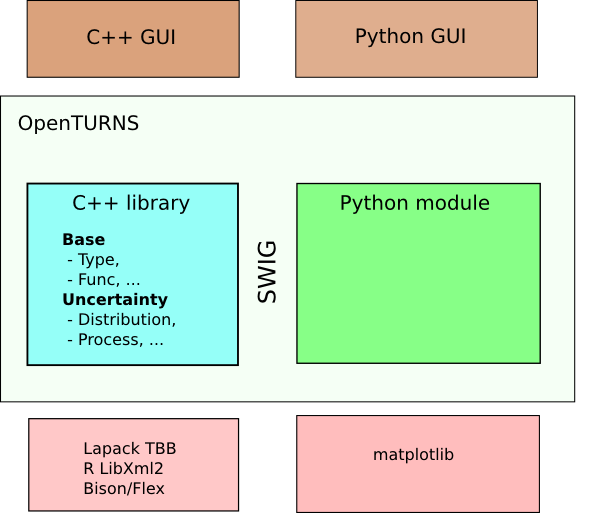
\includegraphics[scale=0.5]{Figures/architecture.png}
\caption{Software architecture overview}
\end{center}
\end{figure}

\subsubsection{The C++ library}

\paragraph{A multi-layered library}

The library has a multi-layered architecture materialized by the source tree.
The two main layers in the C++ library are the Base layer and the Uncertainty layer.
\begin{itemize}
\item Base layer: it contains all the classes not related to the probabilistic concepts. It covers the elementary data types (vectors as NumericalPoint, samples as NumericalSamples), the concept of models (NumericalMathFunction), the linear algebra (Matrix, Tensor) and the general interest classes (memory management, resource management);
\item Uncertainty layer: it contains all the classes that deal with probabilistic concepts. It covers the probabilistic modelling (Distribution, RandomVector), the stochastic algorithms (MonteCarlo, FORM), the statistical estimation (DistributionFactory), the statistical testing (FittingTest)
\end{itemize}
A class in the Uncertainty layer can use any class in the Base or the Uncertainty layer. A class in the Base layer can ONLY USE classes in the Base layer.

\paragraph{Resource management}

OpenTURNS uses extensively dynamic memory allocation. In order to tie to the Resource Acquisition Is Initialization (RAII) paradigm, all the memory management is delegated to smart pointers (the Pointer class). The benefits of this approach are:
\begin{itemize}
\item An easy to implement copy on write mechanism, that permit a significant reduction of the memory footprint by allowing for a large data sharing between objects;
\item No C-like pointers in members of classes, which permits an automatic generation of the copy constructor, the assignment operator and the destructor of almost all the classes: there is no problem of deep copy versus reference copy;
\item The resource is released automatically when the objects are outside of the current scope and there is no more reference on the allocated memory;
\item There is a unique point where to prevent concurrent access in a parallel context, which is a key property for parallelism.
\end{itemize}

\subsubsection{The Python module}

The binding of the library is done almost automatically by SWIG (Simplified Wrapper Interface Generator) through a set of SWIG interface files (.i).\\
The main target language is python.
These swig files contain some specific 'glue code' to each class for the target script language.
SWIG parses the library headers and theses swig interface files to generates the corresponding module source yet to be compiled to produce a binary python module, see \ref{fig:swig}.
The process is shared between several modules for modularity and to speed up compilation time with parallel builds.

\begin{figure}[H]
\begin{center}
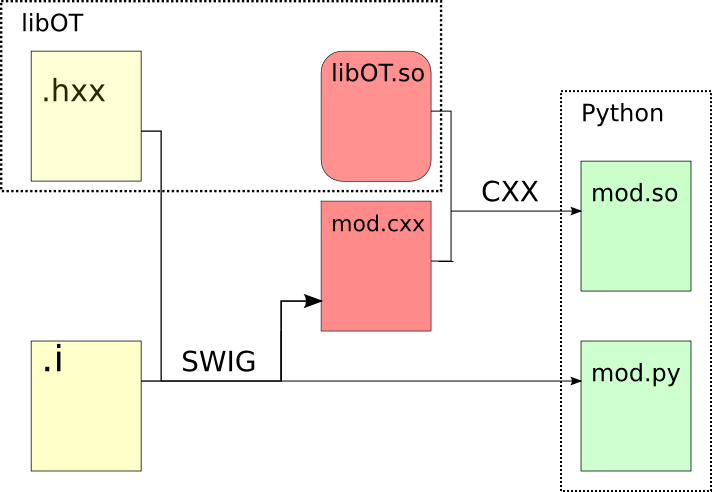
\includegraphics[scale=0.5]{Figures/design/swig.png}
\caption{Python module generation process}\label{fig:swig}
\end{center}
\end{figure}

\subsection{Software environment}

This section details the technical elements required by the OpenTURNS platform, namely the system requirements, the tools and the development environment of the project.

\subsubsection{Target platforms}

The OpenTURNS platform is meant to carry out uncertainty treatment studies in a scientific environment. Most of the scientific codes being available on Unix platforms, OpenTURNS is naturally designed to run on this family of systems. Unix being a standard with multiple implementations, available on different architectures, this gives a wide choice of target platforms.

Linux is currently the most attractive Unix system for the OpenTURNS project, it was chosen as the main target system for the project's development as well as for the delivery of the different versions.

The partners involved in the project have each chosen different Linux distributions, for technical and historical reasons. Therefore, it was decided to support several distributions, a choice that should not be seen as final or minimal. The distributions considered here include for example the list given in Table \ref{linux}

\begin{center}
\begin{table}[h]
\caption{\label{linux}Operating systems supported by the project's partners}
\begin{center}
\begin{tabular}{|l|l|}
\hline
\textbf{Distribution} & \textbf{Version} \\
\hline \hline
Debian & 6 "Squeeze" \\
Ubuntu & 12.04 "Precise" \\
Windows & XP \\
Windows & 7 \\
\hline
\end{tabular}
\end{center}
\end{table}
\end{center}

The primary development platform is Linux, and is known to work on various other distributions.

The Windows version is obtained by cross-compilation using MinGW.

\subsubsection{Dependencies}

The tools chosen for the development of the platform are listed in Table \ref{tools}

\begin{center}
\begin{table}[h]
\caption{\label{tools}Software development tools}
\begin{center}
\begin{tabular}{|l|l|l|}
\hline
\textbf{Category} & \textbf{Name} & \textbf{Version} \\
\hline \hline
Configuration & CMake & 2.8 or later \\
C/C++/Fortran compiler & Gcc & 3.3.5 or later \\
Linear algebra & BLAS & 3.0 or later \\
Linear algebra & LAPACK & 3.0 or later \\
Analytical parser (optional) & muParser & 1.32 or later \\
Distribution functions (optional) & Boost & 1.46 or later \\
CSV parser (optional) & flex & 2.5.33 or later \\
CSV parser (optional) & bison & 2.4 or later \\
XML support (optional) & LibXml2 & 2.6.27 \\
Multithreading (optional) & TBB & 2 or later \\
Python support & Python & 2.3.5 or later \\
Plotting library (optional) & matplotlib & 1.1 or later \\
C++/Python wrapper & SWIG & 1.3.35 or later \\
Statistics library (optional) & R & 2.0.1 or later \\
Calculator (optional for some test) & bc & 1.06 or later \\
Version control & Subversion & 1.1 or later \\
LaTeX to XML (optional for doc) & Tralics & 2.14.5 or later \\
\hline
\end{tabular}
\end{center}
\end{table}
\end{center}

The versions given here are only meant as indications and other versions may be used. However, in case of compatibility issues arising from the use of other packages than those suggested here, support may not be the responsibility of the project.

\subsubsection{Compilation infrastructure}

The historic autotools compilation infrastructure was replaced by CMake. CMake is a lot faster, and the resulting infrastructure is easier to maintain. It covers:
\begin{itemize}
\item The detection and configuration aspects of the platform;
\item The dependency management of the sources;
\item The generation of parallel makefiles;
\item The regression tests.
\end{itemize}
CMake could also provide a way to compile the Windows version using Microsoft compilers.

\subsubsection{Packaging}

The \OT\ team officially provides binaries for the Debian operating system, and Windows.
Note that \OT\ is officially supported in Debian: it can be installed easily from the debian software repositories.
Experimental packages may be available for some RPM-based distributions such as Fedora, CentOS and OpenSUSE.

\subsubsection{Autobuilder}

\OT\ provides developers with a continuous integration environment.
It consists in an daemon monitoring the version control software for changes.
It assumes new code to be involved in regression test.
Also developers should regularly commit to the code base to ensure the origin of a problem is quickly detected.

The autobuilder is triggered by the keyword '\verb|distcheck ok|' in the commit log.

The current test environment consists of the build on each of these platforms:
\begin{itemize}
\item debian 6 x86\_64
\item debian 6 i686
\item windows i686 (wine)
\end{itemize}
The result of the autobuilder made public to anyone registered to the mailing list \verb|commits@openturns.org|.
A summary of each build is provided by mail with links to the logs stored on the server.

\subsection{Design patterns}

\subsubsection{Introduction}

Software design shows the recurrence of some patterns, whether within the same piece of software or in several applications (which can differ in many ways). These patterns have been catalogued, described and implemented in numerous situations that prove their universality and their ability to solve recurring problems that the software architect is faced with.

The following sections give an overview intended as much for the reader's understanding of the document as to establish a common vocabulary for software architect. The latter ones will find here standard design diagrams applied to the specific case of \OT, which can help them better apprehend the tool's specificities and the design and implementation choices that were made.

\label{bridge}\subsubsection{Bridge pattern}

The bridge pattern is a design pattern used in software engineering which is meant to "decouple an abstraction from its implementation so that the two can vary independently". The bridge uses encapsulation, aggregation, and can use inheritance to separate responsibilities into different classes.\\
When a class varies often, the features of object-oriented programming become very useful because changes to a program's code can be made easily with minimal prior knowledge about the program. The bridge pattern is useful when both the class as well as what it does vary often. The class itself can be thought of as the implementation and what the class can do as the abstraction. The bridge pattern can also be thought of as two layers of abstraction.

This pattern is one of the most widely used in \OT. Some examples are:
\begin{itemize}
\item Drawable, that separate the generic high level interface of a drawable from the specific low level interface of the several drawable specializations;
\item Distribution, see \ref{fig:bridge}, that exposes a high level interface of the concept of probability distribution whereas the DistributionImplementation class exposes the low level interface of the same concept.
\end{itemize}

\begin{figure}[htb]
\begin{center}
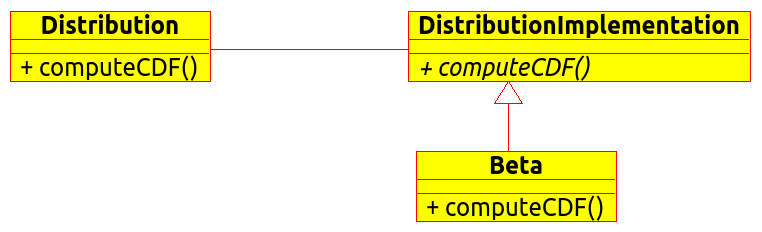
\includegraphics[scale=0.5]{Figures/modeling_notions/bridge.png}
\caption{Bridge pattern example.}\label{fig:bridge}
\end{center}
\end{figure}


\label{singleton}\subsubsection{Singleton pattern}

The Singleton is a pattern used to ensure that at any given time, there is only one instance of a class (A); it provides an access point for this unique instance.

This is implemented by creating a class (Singleton) with a static private attribute (uniqueInstance) initialized with an instance of class A and whose reference (or pointer) is returned by a static method (instance). Figure \ref{fig:singleton} illustrates the Singleton pattern.

\begin{figure}[htb]
\begin{center}
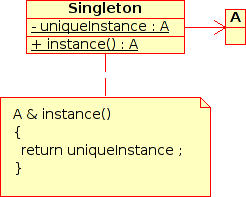
\includegraphics[scale=0.5]{Figures/modeling_notions/singleton.png}
\caption{Singleton structure.}\label{fig:singleton}
\end{center}
\end{figure}

It is a very common pattern that allows to find and share an object (which must remain unique) in different portions of code.
Examples of such objects include shared hardware resources (standard output, error, log, etc.), but also internal functions that cannot or must not be duplicated (e.g. a random number generator).
For example, the classes ResourceMap and IdFactory follow this pattern.

\label{factory}\subsubsection{Factory pattern}

This pattern allows to define a unique interface for the creation of objects belonging to a class hierarchy without knowing in advance their exact type.
Figure \ref{fig:factory} illustrates this pattern.
The creation of the concrete object (ClassA or ClassB) is delegated to a sub-class (ClassAFactory or ClassBFactory) which chooses the type of object to be created and the strategy to be used to create it.

\begin{figure}[htb]
\begin{center}
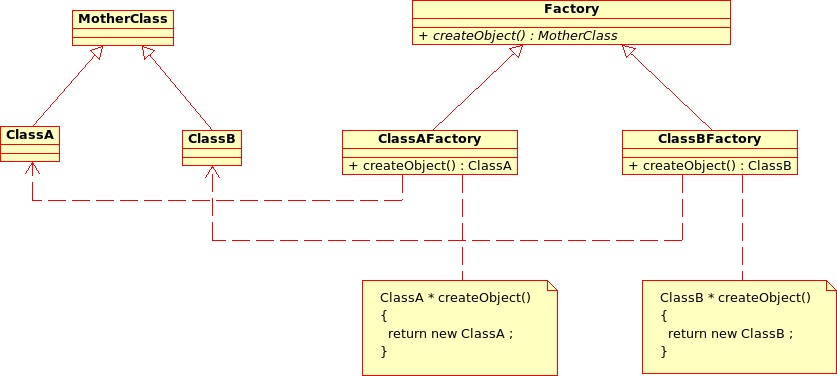
\includegraphics[scale=0.5]{Figures/modeling_notions/factory.png}
\caption{Factory structure.}\label{fig:factory}
\end{center}
\end{figure}

This pattern is often used to dynamically create objects belonging to related types (e.g. to instantiate objects within a GUI according to the user's behavior).
It can also be used to back up and read again a document written in a file by automatically re-instantiating objects.
It is a pattern that makes code maintenance easier by clearly separating the objects and their instantiation in distinct and parallel class hierarchies.
For example, the classes DistributionFactory, ApproximationAlgorithmImplementationFactory, BasisSequenceFactory follow this pattern.

\label{strategy}\subsubsection{Strategy pattern}

The Strategy pattern defines a family of algorithm and makes them interchangeable as far as the client is concerned. Access to these algorithms is provided by a unique interface which encapsulates the algorithms' implementation. Therefore, the implementation can change without the client being aware of it.

\begin{figure}[htb]
\begin{center}
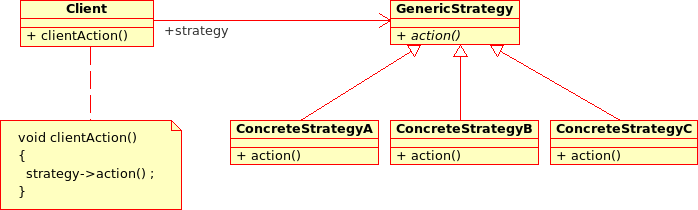
\includegraphics[scale=0.5]{Figures/modeling_notions/strategy.png}
\caption{Strategy structure.}\label{fig:strategy}
\end{center}
\end{figure}

This pattern is very useful to provide a client with different implementations of an algorithm which are equivalent from a functional point of view. It can be noted that the Factory pattern described earlier makes use of the Strategy pattern.
For example, the classes ComparisonOperator, HistoryStrategy follow this pattern.

\label{composite}\subsubsection{Composite pattern}

The Composite pattern is used to organize objects into a tree structure that represents the hierarchies between component and composite objects. It hides the complex structure of the object from the client handling the object.

\begin{figure}[htb]
\begin{center}
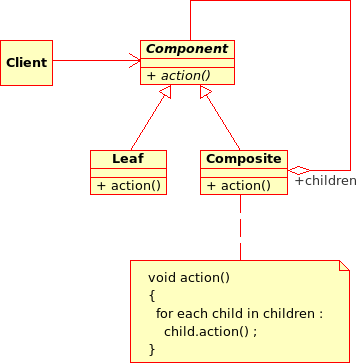
\includegraphics[scale=0.5]{Figures/modeling_notions/composite.png}
\caption{Composite structure.}\label{fig:composite}
\end{center}
\end{figure}

Figure \ref{fig:composite_tree} shows an example of tree modeled by the Composite. The Composite objects make up the tree nodes whereas the leaves can be any concrete object deriving from Component.

\begin{figure}[htb]
\begin{center}
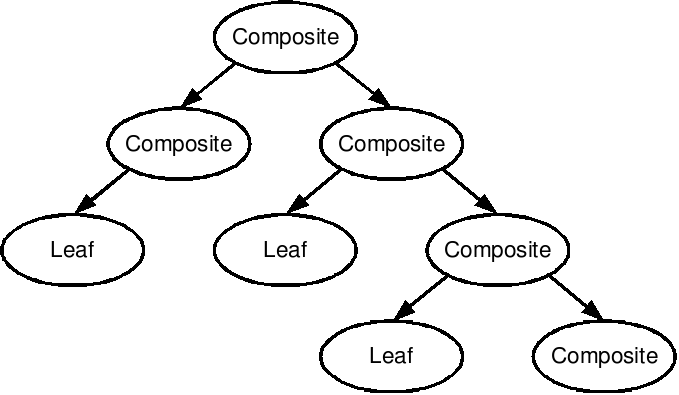
\includegraphics[scale=0.45]{Figures/modeling_notions/composite_tree.png}
\caption{Example of tree modeled by the Composite.}\label{fig:composite_tree}
\end{center}
\end{figure}

The Composite pattern is an essential element of the design model for the \OT\ platform. It can be used to model numerical function composition, random vector composition, etc. It can be found in several aspects of the modeling brick. Any related objects tree structure can rely on the Composite pattern with benefit.
For example, the classes ComposedDistribution, CompositeRandomVector, ComposedNumericalMathFunction follow this pattern.
